\documentclass{article}
\usepackage{lmodern}
\usepackage[charter]{mathdesign}
\usepackage[english]{babel}
\usepackage[utf8]{inputenc}

\usepackage{caption,subcaption}
\usepackage{fullpage}
\usepackage{color}
\usepackage{manfnt}
\usepackage{wasysym}
\usepackage{listings}
\usepackage{graphicx}
\usepackage{url}
%\usepackage{ulem}
\usepackage{marvosym}
%\usepackage{skull}
\usepackage{proof}
\usepackage{array}

\title{{\bf Dynamic Scheduling in Halide}}
\author{Ben Blum \texttt{(bblum@andrew.cmu.edu)}}

\date{2013, December 16}

\newcommand\noob{\mathsf{noob}}
\newcommand\gibs{\mathsf{gibs}}
\newcommand\dps{\mathsf{dps}}
\newcommand\squig\rightsquigarrow
\newcommand\Coloneqq{\mathrel{\mathop{::}}=}
\newcommand\dmg{\text{\Laserbeam}}
\newcommand\delter\delta
\newcommand\alpher\alpha
\newcommand\defnor{\text{ }|\text{ }}

\newcommand\pimp{\mathop{\supset}}
\newcommand\pand{\mathop{\wedge}}
\newcommand\por{\mathop{\vee}}
\newcommand\ptrue{\top}
\newcommand\pfalse{\bot}


\begin{document}
\maketitle

\begin{figure}[h]
	\begin{center}
	\begin{tabular}{llllll}
		\begin{tabular}{l}
                \texttt{blur\_y(x,y) =} \\
                \texttt{~~~~(input(x, y-1) +}\\
                \texttt{~~~~~input(x, y~~) +}\\
                \texttt{~~~~~input(x, y+1))/3;}\\
                \\
                \texttt{blur\_x(x,y) =} \\
                \texttt{~~~~(blur\_y(x-1, y) +}\\
                \texttt{~~~~~blur\_y(x,~~~y) +}\\
                \texttt{~~~~~blur\_y(x+1, y))/3;}\\
		\end{tabular}
		& & & & &
		\begin{tabular}{l}
                \texttt{blur\_y\_far\_away(x,y) =} \\
                \texttt{~~~~(input(x, {\bf y-rand()}) +}\\
                \texttt{~~~~~input(x, y~~~~~~~) +}\\
                \texttt{~~~~~input(x, {\bf y+rand()}))/3;}\\
                \\
                \texttt{blur\_x\_far\_away(x,y) =} \\
                \texttt{~~~~(blur\_y({\bf x-rand()}, y) +}\\
                \texttt{~~~~~blur\_y(x,~~~~~~~~y) +}\\
                \texttt{~~~~~blur\_y({\bf x+rand()}, y))/3;}\\
		\end{tabular}

	\end{tabular}
	\end{center}
	\caption{Static and dynamic data dependencies in Halide. On the left, a 3x3 blur (the canonical example Halide program) need only reference input data up to 1 pixel away in each direction for each output pixel. On the right, the algorithm is modified such that the compiler cannot statically know which input pixels each output pixel may reference.}
	\label{fig:intro}
\end{figure}

%%%%%%%%%%%%%%%%%%%%%%%%%%%%%%%%%%%%%%%%%%%%%%%%%%%%%%%%%%%%%%%%%%%%%%%%%%%%%%%%
\section{Introduction}

Halide~\cite{halide} is a programming language for image processing pipelines designed to separate the concerns of performance and expressivity. The programming model is functional, representing images as functions from pixel coordinates to colour values, and representing each pass of an image processing algorithm as a function from images to images. Once implemented, the programmer's algorithm is then automatically parallelized by the Halide runtime, taking into account considerations such as how to split each pass into parallel tiles and the data dependencies between two consecutive passes.
The structure of the generated loop nest and the function calls therein is known as the {\em function schedule}.

One weakness of Halide is its inability to express image processing passes that don't operate uniformly across their domain; i.e., algorithms whose data dependencies on portions of previous passes cannot be known statically.
Figure~\ref{fig:intro} above contrasts two simple example algorithms, showcasing the difference between static and dynamic data dependencies.

In this project I investigate and implement {\em dynamic function scheduling}, a new language feature for Halide to support such algorithms.
My approach allows the computations for early pipeline stages to be cached across loop iterations of later stages, so that the results may be reused when data dependencies happen to coincide on the same location, saving redundant computation of a possibly expensive intermediate function.
The principal contribution of this work is the implementation and performance evaluation of {\em dynamic scheduling at pixel granularity}. I also investigated dynamic scheduling at coarser (e.g. tile) granularities, with which entire loop iterations may be skipped. However, the problem was more difficult than anticipated, so I instead provide some discussion and a design sketch for future work.

%%%%%%%%%%%%%%%%%%%%%%%%%%%%%%%%%%%%%%%%%%%%%%%%%%%%%%%%%%%%%%%%%%%%%%%%%%%%%%%%
\section{Motivation}

\definecolor{grey}{RGB}{127,127,127}
\definecolor{darkcyan}{RGB}{0,127,127}
\definecolor{olivegreen}{RGB}{0,127,0}
\definecolor{violet}{RGB}{127,0,127}
\definecolor{brickred}{RGB}{127,0,0}
\definecolor{brown}{RGB}{127,63,0}
\definecolor{orange}{RGB}{192,96,0}
\newcommand\hilight[2]{\color{#1}#2\color{black}}


\begin{figure}[t]
	\begin{center}
	\begin{subfigure}[b]{0.45\textwidth}
		\begin{center}
		\begin{tabular}{l}
		{\em User-provided schedule:} \\
		\\
		\hilight{blue}{\texttt{blur\_x /* nothing special */;}} \\
		\hilight{olivegreen}{\texttt{blur\_y.store\_root().compute\_root();}} \\
		\\
		{\em Compiler-generated code:} \\
		\\
                \texttt{\hilight{olivegreen}{float~blur\_y[HEIGHT][WIDTH];}} \\
                \texttt{\hilight{olivegreen}{for~(row~=~0~to~HEIGHT)~\{}} \\
                \texttt{\hilight{olivegreen}{~~for~(col~=~0~to~WIDTH)~\{}} \\
                \texttt{\hilight{olivegreen}{~~~~blur\_y[row][col] = ...;}}\\
                \texttt{\hilight{olivegreen}{~~\}}} \\
                \texttt{\hilight{olivegreen}{\}}} \\
		\\
                \texttt{\hilight{blue}{float~blur\_x[HEIGHT][WIDTH];}} \\
                \texttt{\hilight{blue}{for~(row~=~0~to~HEIGHT)~\{}} \\
                \texttt{\hilight{blue}{~~for~(col~=~0~to~WIDTH)~\{}} \\
                \texttt{\hilight{blue}{~~~~blur\_x[row][col] = ...;}}\\
                \texttt{\hilight{blue}{~~\}}} \\
                \texttt{\hilight{blue}{\}}} \\
		\end{tabular}
		\end{center}
		\caption{\texttt{blur\_x} and \texttt{blur\_y} are scheduled separately. This schedule, while easy to understand, offers poor locality (values computed are not used until a full image traversal later) and poor parallelism (creating one thread per row or column of pixels both floods the system with too many threads and creates cache contention).}
		\label{fig:scheds-a}
	\end{subfigure}
	\qquad
	\begin{subfigure}[b]{0.5\textwidth}
		\begin{center}
		\begin{tabular}{l}
		{\em User-provided schedule:} \\
		\\
                \hilight{blue}{\texttt{blur\_x.tile(x, y, x2, y2, 8, 8).parallel(y);}}\\
                \hilight{olivegreen}{\texttt{blur\_y.store\_at(blur\_x, x).compute\_at(blur\_x, y2);}}\\
                \\
		{\em Compiler-generated code:} \\
		\\
                \texttt{\hilight{blue}{float~blur\_x[HEIGHT][WIDTH];}} \\
                \texttt{\hilight{blue}{PARALLEL for~(row~=~0~to~8)~\{}} \\
                \texttt{\hilight{blue}{~~for~(col~=~0~to~8)~\{}} \\
                \texttt{\hilight{olivegreen}{~~~~float~blur\_y[HEIGHT/8 + 2][WIDTH/8 + 2];}} \\
                \texttt{\hilight{blue}{~~~~for~(row2~=~0~to~WIDTH/8 + 2)~\{}} \\
                \texttt{\hilight{olivegreen}{~~~~~~for~(col2~=~0~to~WIDTH/8 + 2)~\{}} \\
                \texttt{\hilight{olivegreen}{~~~~~~~~blur\_y[row2][col2]~=~...;}} \\
                \texttt{\hilight{olivegreen}{~~~~~~\}}} \\
                \texttt{\hilight{blue}{~~~~~~for~(col2~=~0~to~WIDTH/8)~\{}} \\
                \texttt{\hilight{blue}{~~~~~~~~blur\_x[row*8~+~row2][col*8~+~col2]~=~...;}} \\
                \texttt{\hilight{blue}{~~~~~~\}}} \\
                \texttt{\hilight{blue}{~~~~\}}} \\
                \texttt{\hilight{blue}{~~\}}} \\
                \texttt{\hilight{blue}{\}}} \\
		\end{tabular}
		\end{center}
		\caption{\texttt{blur\_x} is tiled in 8-fold splits in each dimension, and \texttt{blur\_y} is scheduled at the tile level within \texttt{blur\_x}. This schedule offers good locality (values are used soon after being computed) and good parallelism (one thread per tile; tile size can be customized).}
		\label{fig:scheds-b}
	\end{subfigure}
	\end{center}
	\caption{Two example function schedules for the two-stage blur algorithm shown in Figure~\ref{fig:intro}.}
	\label{fig:scheds}
\end{figure}

The high concept of Halide is to separate the logic of an image processing algorithm from the order in which the functions for each stage are scheduled. Figure~\ref{fig:scheds} shows two possible schedules for our example algorithm, and discusses the performance characteristics of each.
Though Figure~\ref{fig:scheds-b} is more cache-friendly and offers superior paralellism opportunity, a notable disadvantage is that some computation is duplicated across tiles. This is shown in the extra 2 pixels computed for \texttt{blur\_y} in each dimension. In this example, the overhead is minor, as Halide can statically reason about the maximum extra ``padding'' that \texttt{blur\_y} must compute for each tile of \texttt{blur\_x}.

However, this extra computation can become a significant problem when the dependencies between the algorithm's stages are computed at runtime and hence are not available for compile-time reasoning, as in the PatchMatch algorithm~\cite{patchmatch} and in edge detection. If the user wishes to use a cache-friendly, highly-parallel function schedule, as in Figure~\ref{fig:scheds-b}, Halide must make a conservative estimate regarding how much extra padding is required, resulting in extra work duplication.

To get a sense for how much extra unnecessary computation can arise, we introduce a sample two-stage Halide program in which the second stage (\texttt{flip()}) dynamically computes which pixels it requires from the first stage (\texttt{invert()}). This program is described in Figure~\ref{fig:flip}. We then ran this program on a test image using the simple schedule from Figure~\ref{fig:scheds-a} and using several nested schedules as in Figure~\ref{fig:scheds-b}. We found that in the former situation, 13,068 calls to \texttt{invert()} were required, while in the latter, \texttt{invert()} was invoked anywhere between 252,648 to 7,847,400 times depending on the schedule used.
Hence, the motivation for {\em dynamic scheduling} is to extend Halide's ability to avoid duplicate work to apply to this wider range of algorithms.

\begin{figure}[t]
	\begin{tabular}{cc}
	\begin{subfigure}[b]{0.45\textwidth}
		\begin{center}
		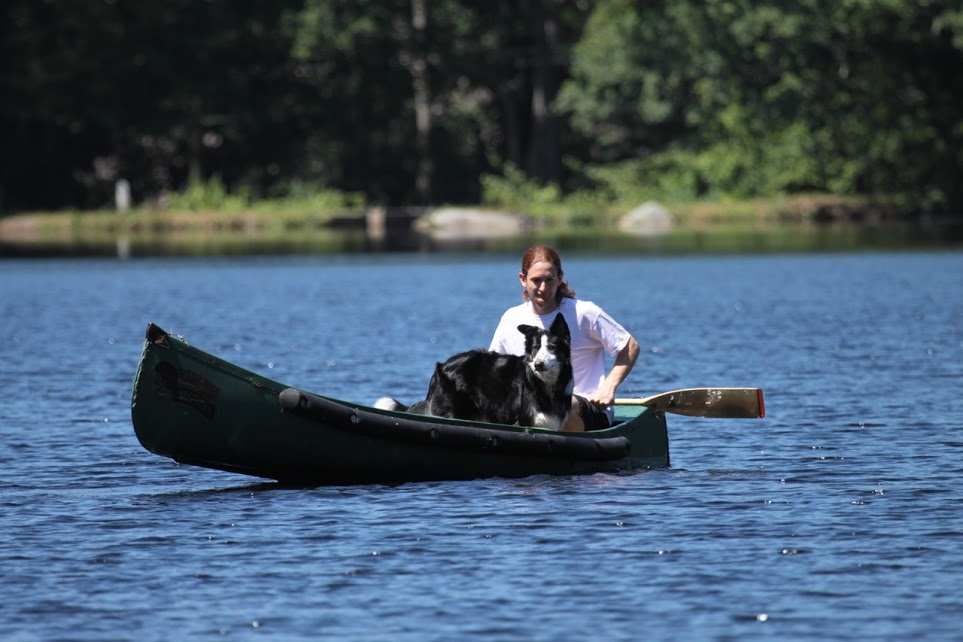
\includegraphics[width=0.85\textwidth]{canoe-0.png}
		\end{center}
		\caption{Original input image.}
	\end{subfigure} &
	\begin{subfigure}[b]{0.45\textwidth}
		\begin{center}
		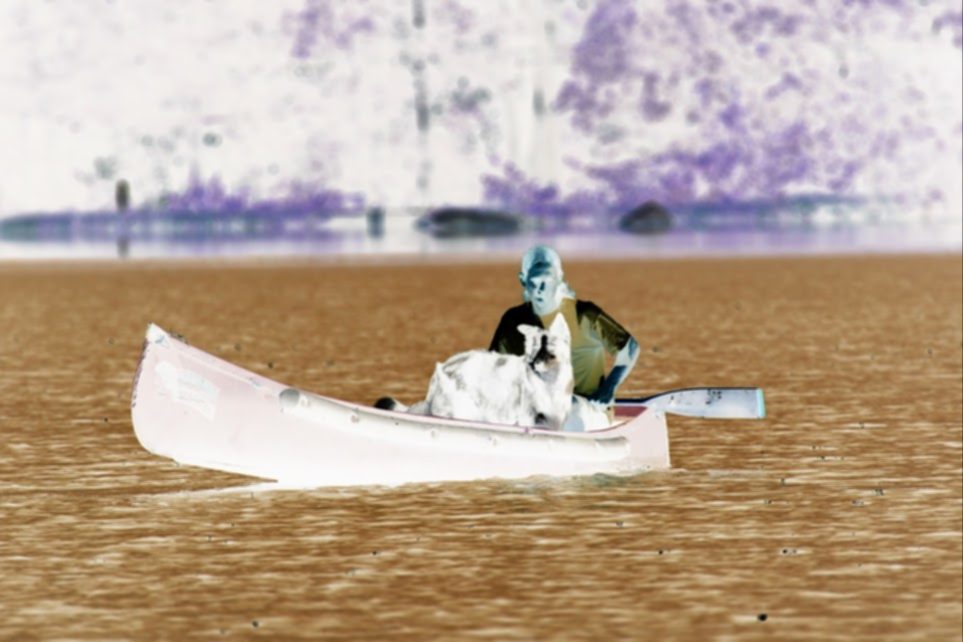
\includegraphics[width=0.85\textwidth]{canoe-1.png}
		\end{center}
		\caption{Stage 1 is a simple value-invert of each input pixel.}
		\label{fig:invert}
	\end{subfigure} \\
	& \\
	\begin{subfigure}[b]{0.45\textwidth}
		\begin{center}
		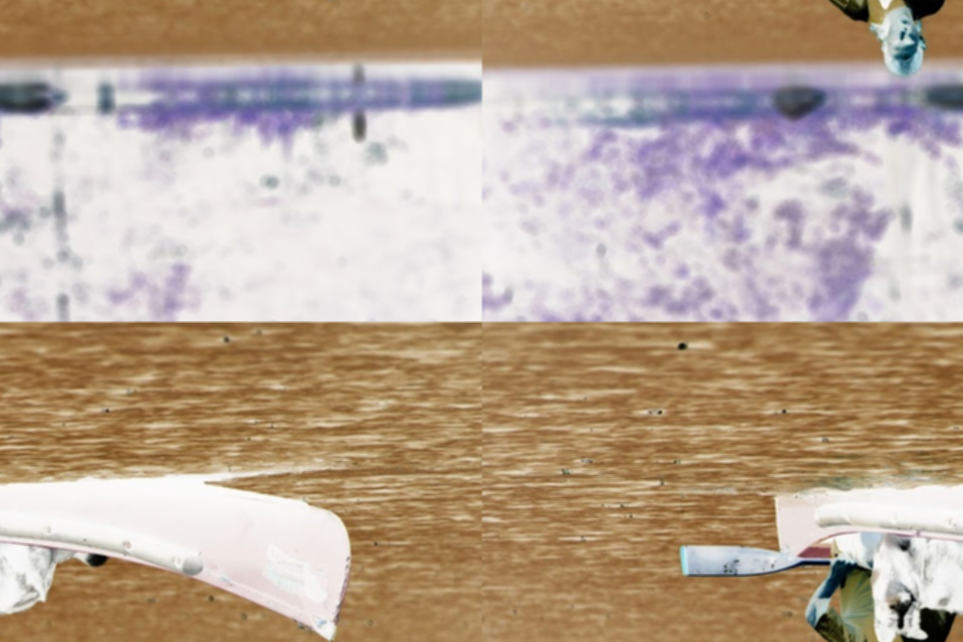
\includegraphics[width=0.85\textwidth]{canoe-2.png}
		\end{center}
		\caption{The core of stage 2 is a transformation across a vector field, which maps points near the center to the corners and points near the corners to the center, followed by a 3x3 blur. The blur causes each output pixel to depend on multiple input pixels, which allows for the possibility of work duplication.}
		\label{fig:flip-blur-1}
	\end{subfigure} &
	\begin{subfigure}[b]{0.45\textwidth}
		\begin{center}
		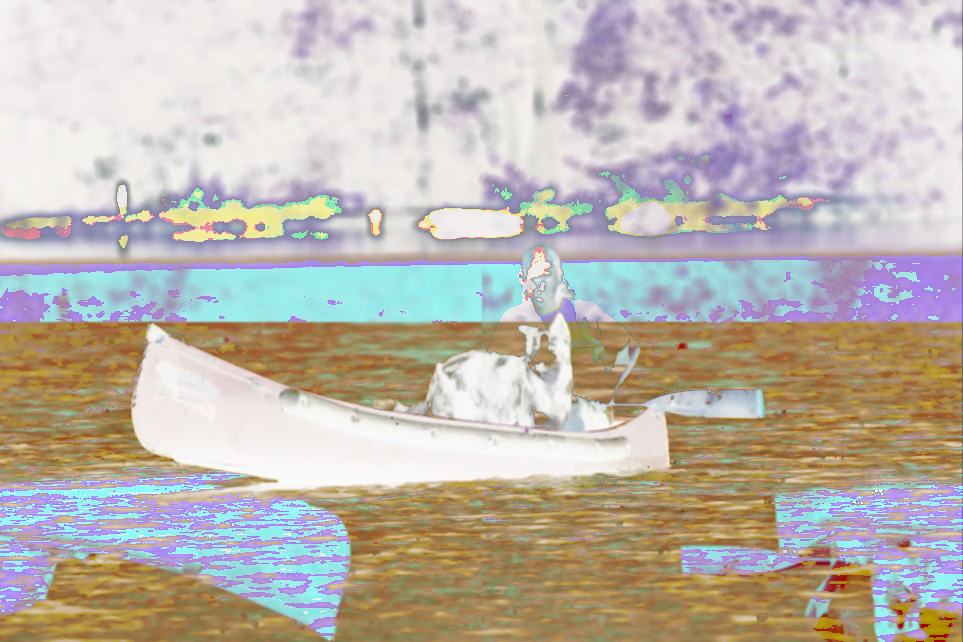
\includegraphics[width=0.85\textwidth]{canoe-3.png}
		\end{center}
		\caption{Final output. Stage 2 is altered to only apply the vector field to pixels when their colour value is darker than a certain threshold. This condition, which depends on a nondeterministic property of the input image, prevents Halide's optimizations from reasoning about the data dependencies between the two stages.}
		\label{fig:flip-blur-2}
	\end{subfigure}
	\end{tabular}
	\caption{Our sample image processing program consists of two stages, \texttt{invert()} (shown in \ref{fig:invert}) and \texttt{flip()} (shown in \ref{fig:flip-blur-1} and \ref{fig:flip-blur-2}). We designed this program expressly to create dynamic data dependencies with wide ranges across the image, to ensure a static function schedule could not avoid duplicating work.}

	\label{fig:flip}
\end{figure}

%%%%%%%%%%%%%%%%%%%%%%%%%%%%%%%%%%%%%%%%%%%%%%%%%%%%%%%%%%%%%%%%%%%%%%%%%%%%%%%%
\section{Design and Interface}
% TODO

%%%%%%%%%%%%%%%%%%%%%%%%%%%%%%%%%%%%%%%%%%%%%%%%%%%%%%%%%%%%%%%%%%%%%%%%%%%%%%%%
\section{Implementation}

\subsection{Code Generation}
% TODO

\subsection{Legality Checking}
% TODO

\subsection{Code}

The reader should feel free to find and peruse my code at \texttt{https://github.com/bblum/Halide}. During the weeks following this submission I will polish it and submit a pull request upstream.

%%%%%%%%%%%%%%%%%%%%%%%%%%%%%%%%%%%%%%%%%%%%%%%%%%%%%%%%%%%%%%%%%%%%%%%%%%%%%%%%
\section{Evaluation}
% TODO

%%%%%%%%%%%%%%%%%%%%%%%%%%%%%%%%%%%%%%%%%%%%%%%%%%%%%%%%%%%%%%%%%%%%%%%%%%%%%%%%
\section{Open Questions}
% TODO

%%%%%%%%%%%%%%%%%%%%%%%%%%%%%%%%%%%%%%%%%%%%%%%%%%%%%%%%%%%%%%%%%%%%%%%%%%%%%%%%
\section{Conclusion}
% TODO

%%%%%%%%%%%%%%%%%%%%%%%%%%%%%%%%%%%%%%%%%%%%%%%%%%%%%%%%%%%%%%%%%%%%%%%%%%%%%%%%
\section*{Acknowledgements}

Thanks to Jonathan Ragan-Kelley and Andrew Adams, developers of Halide, for their guidance, insights, and patience. Thanks to Kayvon Fatahalian for supervising this project and for a great semester in 15-869.

\bibliography{citations}{}
\bibliographystyle{alpha}
\end{document}

%%%%%%%%%%%%%%%%%%%%%%%%%%%%%%%%%%%%%%%%%%%%%%%%%%%%%%%%%%%%%%%%%%%%%%%%%%%%%%%%
% vim: foldmethod=indent
